\documentclass[]{article}
\usepackage{lmodern}
\usepackage{amssymb,amsmath}
\usepackage{ifxetex,ifluatex}
\usepackage{fixltx2e} % provides \textsubscript
\ifnum 0\ifxetex 1\fi\ifluatex 1\fi=0 % if pdftex
  \usepackage[T1]{fontenc}
  \usepackage[utf8]{inputenc}
\else % if luatex or xelatex
  \ifxetex
    \usepackage{mathspec}
  \else
    \usepackage{fontspec}
  \fi
  \defaultfontfeatures{Ligatures=TeX,Scale=MatchLowercase}
\fi
% use upquote if available, for straight quotes in verbatim environments
\IfFileExists{upquote.sty}{\usepackage{upquote}}{}
% use microtype if available
\IfFileExists{microtype.sty}{%
\usepackage{microtype}
\UseMicrotypeSet[protrusion]{basicmath} % disable protrusion for tt fonts
}{}
\usepackage[margin=1in]{geometry}
\usepackage{hyperref}
\hypersetup{unicode=true,
            pdftitle={Basic Concepts of Exploratory Analysis},
            pdfborder={0 0 0},
            breaklinks=true}
\urlstyle{same}  % don't use monospace font for urls
\usepackage{color}
\usepackage{fancyvrb}
\newcommand{\VerbBar}{|}
\newcommand{\VERB}{\Verb[commandchars=\\\{\}]}
\DefineVerbatimEnvironment{Highlighting}{Verbatim}{commandchars=\\\{\}}
% Add ',fontsize=\small' for more characters per line
\usepackage{framed}
\definecolor{shadecolor}{RGB}{248,248,248}
\newenvironment{Shaded}{\begin{snugshade}}{\end{snugshade}}
\newcommand{\KeywordTok}[1]{\textcolor[rgb]{0.13,0.29,0.53}{\textbf{#1}}}
\newcommand{\DataTypeTok}[1]{\textcolor[rgb]{0.13,0.29,0.53}{#1}}
\newcommand{\DecValTok}[1]{\textcolor[rgb]{0.00,0.00,0.81}{#1}}
\newcommand{\BaseNTok}[1]{\textcolor[rgb]{0.00,0.00,0.81}{#1}}
\newcommand{\FloatTok}[1]{\textcolor[rgb]{0.00,0.00,0.81}{#1}}
\newcommand{\ConstantTok}[1]{\textcolor[rgb]{0.00,0.00,0.00}{#1}}
\newcommand{\CharTok}[1]{\textcolor[rgb]{0.31,0.60,0.02}{#1}}
\newcommand{\SpecialCharTok}[1]{\textcolor[rgb]{0.00,0.00,0.00}{#1}}
\newcommand{\StringTok}[1]{\textcolor[rgb]{0.31,0.60,0.02}{#1}}
\newcommand{\VerbatimStringTok}[1]{\textcolor[rgb]{0.31,0.60,0.02}{#1}}
\newcommand{\SpecialStringTok}[1]{\textcolor[rgb]{0.31,0.60,0.02}{#1}}
\newcommand{\ImportTok}[1]{#1}
\newcommand{\CommentTok}[1]{\textcolor[rgb]{0.56,0.35,0.01}{\textit{#1}}}
\newcommand{\DocumentationTok}[1]{\textcolor[rgb]{0.56,0.35,0.01}{\textbf{\textit{#1}}}}
\newcommand{\AnnotationTok}[1]{\textcolor[rgb]{0.56,0.35,0.01}{\textbf{\textit{#1}}}}
\newcommand{\CommentVarTok}[1]{\textcolor[rgb]{0.56,0.35,0.01}{\textbf{\textit{#1}}}}
\newcommand{\OtherTok}[1]{\textcolor[rgb]{0.56,0.35,0.01}{#1}}
\newcommand{\FunctionTok}[1]{\textcolor[rgb]{0.00,0.00,0.00}{#1}}
\newcommand{\VariableTok}[1]{\textcolor[rgb]{0.00,0.00,0.00}{#1}}
\newcommand{\ControlFlowTok}[1]{\textcolor[rgb]{0.13,0.29,0.53}{\textbf{#1}}}
\newcommand{\OperatorTok}[1]{\textcolor[rgb]{0.81,0.36,0.00}{\textbf{#1}}}
\newcommand{\BuiltInTok}[1]{#1}
\newcommand{\ExtensionTok}[1]{#1}
\newcommand{\PreprocessorTok}[1]{\textcolor[rgb]{0.56,0.35,0.01}{\textit{#1}}}
\newcommand{\AttributeTok}[1]{\textcolor[rgb]{0.77,0.63,0.00}{#1}}
\newcommand{\RegionMarkerTok}[1]{#1}
\newcommand{\InformationTok}[1]{\textcolor[rgb]{0.56,0.35,0.01}{\textbf{\textit{#1}}}}
\newcommand{\WarningTok}[1]{\textcolor[rgb]{0.56,0.35,0.01}{\textbf{\textit{#1}}}}
\newcommand{\AlertTok}[1]{\textcolor[rgb]{0.94,0.16,0.16}{#1}}
\newcommand{\ErrorTok}[1]{\textcolor[rgb]{0.64,0.00,0.00}{\textbf{#1}}}
\newcommand{\NormalTok}[1]{#1}
\usepackage{graphicx,grffile}
\makeatletter
\def\maxwidth{\ifdim\Gin@nat@width>\linewidth\linewidth\else\Gin@nat@width\fi}
\def\maxheight{\ifdim\Gin@nat@height>\textheight\textheight\else\Gin@nat@height\fi}
\makeatother
% Scale images if necessary, so that they will not overflow the page
% margins by default, and it is still possible to overwrite the defaults
% using explicit options in \includegraphics[width, height, ...]{}
\setkeys{Gin}{width=\maxwidth,height=\maxheight,keepaspectratio}
\IfFileExists{parskip.sty}{%
\usepackage{parskip}
}{% else
\setlength{\parindent}{0pt}
\setlength{\parskip}{6pt plus 2pt minus 1pt}
}
\setlength{\emergencystretch}{3em}  % prevent overfull lines
\providecommand{\tightlist}{%
  \setlength{\itemsep}{0pt}\setlength{\parskip}{0pt}}
\setcounter{secnumdepth}{0}
% Redefines (sub)paragraphs to behave more like sections
\ifx\paragraph\undefined\else
\let\oldparagraph\paragraph
\renewcommand{\paragraph}[1]{\oldparagraph{#1}\mbox{}}
\fi
\ifx\subparagraph\undefined\else
\let\oldsubparagraph\subparagraph
\renewcommand{\subparagraph}[1]{\oldsubparagraph{#1}\mbox{}}
\fi

%%% Use protect on footnotes to avoid problems with footnotes in titles
\let\rmarkdownfootnote\footnote%
\def\footnote{\protect\rmarkdownfootnote}

%%% Change title format to be more compact
\usepackage{titling}

% Create subtitle command for use in maketitle
\providecommand{\subtitle}[1]{
  \posttitle{
    \begin{center}\large#1\end{center}
    }
}

\setlength{\droptitle}{-2em}

  \title{Basic Concepts of Exploratory Analysis}
    \pretitle{\vspace{\droptitle}\centering\huge}
  \posttitle{\par}
    \author{}
    \preauthor{}\postauthor{}
    \date{}
    \predate{}\postdate{}
  

\begin{document}
\maketitle

This R Notebook file is designated to provide all necessary calculations
used in Power point Presentation.

\subsubsection{1. Preprocessing}\label{preprocessing}

Loading of packages (the output is hidden)

Loading of initial variables

\begin{Shaded}
\begin{Highlighting}[]
\CommentTok{# path to file location ()}
\NormalTok{location <-}\StringTok{ 'D:}\CharTok{\textbackslash{}\textbackslash{}}\StringTok{Demyd}\CharTok{\textbackslash{}\textbackslash{}}\StringTok{Personal}\CharTok{\textbackslash{}\textbackslash{}}\StringTok{R}\CharTok{\textbackslash{}\textbackslash{}}\StringTok{kaggle}\CharTok{\textbackslash{}\textbackslash{}}\StringTok{'} \CommentTok{# enter your path to files required. }
\NormalTok{filename <-}\StringTok{ 'application_test.csv'}
\CommentTok{# load initial data}
\NormalTok{data_all <-}\StringTok{ }\KeywordTok{data.table}\NormalTok{(}\KeywordTok{read.csv}\NormalTok{(}\KeywordTok{paste}\NormalTok{(location, filename, }\DataTypeTok{sep =} \StringTok{""}\NormalTok{)))}
\CommentTok{# select variables used in presentation}
\NormalTok{vars <-}\StringTok{ }\KeywordTok{c}\NormalTok{(}\StringTok{'AMT_INCOME_TOTAL'}\NormalTok{,   }\StringTok{'AMT_CREDIT'}\NormalTok{,   }\StringTok{'AMT_ANNUITY'}\NormalTok{,  }\StringTok{'AMT_GOODS_PRICE'}\NormalTok{,  }\StringTok{'REGION_POPULATION_RELATIVE'}\NormalTok{, }\StringTok{'HOUR_APPR_PROCESS_START'}\NormalTok{)}
\NormalTok{data_vars <-}\StringTok{ }\NormalTok{data_all[, ..vars]}
\end{Highlighting}
\end{Shaded}

\subsubsection{2. Mean calculations}\label{mean-calculations}

\begin{Shaded}
\begin{Highlighting}[]
\CommentTok{# user's functions to calculate Geometric Mean and Harmonic Mean}
\NormalTok{gm <-}\StringTok{ }\ControlFlowTok{function}\NormalTok{(x)\{  x <-}\StringTok{ }\NormalTok{x[}\OperatorTok{!}\KeywordTok{is.na}\NormalTok{(x)]; }\KeywordTok{exp}\NormalTok{(}\KeywordTok{mean}\NormalTok{(}\KeywordTok{log}\NormalTok{(x)))\} }\CommentTok{#Geometric Mean https://www.r-bloggers.com/r-geometric-mean/}
\NormalTok{hm <-}\StringTok{ }\ControlFlowTok{function}\NormalTok{(x)\{}\KeywordTok{harmonic.mean}\NormalTok{(x, }\DataTypeTok{na.rm=}\OtherTok{TRUE}\NormalTok{)\} }\CommentTok{#Harmonic Mean https://www.r-bloggers.com/geometric-and-harmonic-means-in-r/}

\CommentTok{# calculations of different mean types (Arithmetic, Geometric and Harmonic Means - AM, GM, HM)}
\NormalTok{mean_summary <-}\StringTok{ }\KeywordTok{as.data.table}\NormalTok{(}\KeywordTok{rbind}\NormalTok{(}\KeywordTok{apply}\NormalTok{(data_vars, }\DecValTok{2}\NormalTok{, mean, }\DataTypeTok{na.rm =} \OtherTok{TRUE}\NormalTok{), }\KeywordTok{apply}\NormalTok{(data_vars, }\DecValTok{2}\NormalTok{, gm), }\KeywordTok{apply}\NormalTok{(data_vars, }\DecValTok{2}\NormalTok{, hm)))}
\end{Highlighting}
\end{Shaded}

\begin{verbatim}
## Warning in harmonic.mean(x, na.rm = TRUE): some values are <= 0, using
## approximation
\end{verbatim}

\begin{Shaded}
\begin{Highlighting}[]
\NormalTok{mean_summary <-}\StringTok{ }\KeywordTok{cbind}\NormalTok{(}\DataTypeTok{item =} \KeywordTok{c}\NormalTok{(}\StringTok{'Arithmetic Mean'}\NormalTok{, }\StringTok{'Geometric Mean'}\NormalTok{, }\StringTok{'Harmonic Mean'}\NormalTok{), mean_summary)}
\NormalTok{mean_summary[}\DecValTok{1}\NormalTok{, }\DecValTok{4}\NormalTok{] <-}\StringTok{ }\KeywordTok{mean}\NormalTok{(data_vars}\OperatorTok{$}\NormalTok{AMT_ANNUITY[}\OperatorTok{!}\KeywordTok{is.na}\NormalTok{(data_vars}\OperatorTok{$}\NormalTok{AMT_ANNUITY)], }\DataTypeTok{na.rm =} \OtherTok{TRUE}\NormalTok{)}


\CommentTok{# calculation of mode and median}
\NormalTok{mode_median <-}\StringTok{ }\KeywordTok{as.data.table}\NormalTok{(}\KeywordTok{rbind}\NormalTok{(}\KeywordTok{apply}\NormalTok{(data_vars, }\DecValTok{2}\NormalTok{, Mode, }\DataTypeTok{na.rm =} \OtherTok{TRUE}\NormalTok{), }\KeywordTok{apply}\NormalTok{(data_vars, }\DecValTok{2}\NormalTok{, median, }\DataTypeTok{na.rm =} \OtherTok{TRUE}\NormalTok{)))}
\NormalTok{mode_median <-}\StringTok{ }\KeywordTok{cbind}\NormalTok{(}\DataTypeTok{item =} \KeywordTok{c}\NormalTok{(}\StringTok{'mode'}\NormalTok{, }\StringTok{'median'}\NormalTok{), mode_median)}
\NormalTok{mode_median[}\DecValTok{1}\NormalTok{, }\DecValTok{4}\NormalTok{] <-}\StringTok{ }\KeywordTok{median}\NormalTok{(data_vars}\OperatorTok{$}\NormalTok{AMT_ANNUITY[}\OperatorTok{!}\KeywordTok{is.na}\NormalTok{(data_vars}\OperatorTok{$}\NormalTok{AMT_ANNUITY)], }\DataTypeTok{na.rm =} \OtherTok{TRUE}\NormalTok{)}

\CommentTok{# calculation of ration AM to Mode/Median}
\NormalTok{am_mode <-}\StringTok{ }\KeywordTok{cbind}\NormalTok{(}\DataTypeTok{item =} \StringTok{'AM/Mode'}\NormalTok{, mean_summary[}\DecValTok{1}\NormalTok{, ..vars] }\OperatorTok{/}\StringTok{ }\NormalTok{mode_median[}\DecValTok{1}\NormalTok{, ..vars])}
\NormalTok{am_median <-}\StringTok{ }\KeywordTok{cbind}\NormalTok{(}\DataTypeTok{item =} \StringTok{'AM/Median'}\NormalTok{, mean_summary[}\DecValTok{1}\NormalTok{, ..vars] }\OperatorTok{/}\StringTok{ }\NormalTok{mode_median[}\DecValTok{1}\NormalTok{, ..vars])}

\CommentTok{# min and max values}
\NormalTok{min_max <-}\StringTok{ }\KeywordTok{as.data.table}\NormalTok{(}\KeywordTok{rbind}\NormalTok{(}\KeywordTok{apply}\NormalTok{(data_vars, }\DecValTok{2}\NormalTok{, min, }\DataTypeTok{na.rm =} \OtherTok{TRUE}\NormalTok{), }\KeywordTok{apply}\NormalTok{(data_vars, }\DecValTok{2}\NormalTok{, max, }\DataTypeTok{na.rm =} \OtherTok{TRUE}\NormalTok{)))}
\NormalTok{min_max <-}\StringTok{ }\KeywordTok{cbind}\NormalTok{(}\DataTypeTok{item =} \KeywordTok{c}\NormalTok{(}\StringTok{'min'}\NormalTok{, }\StringTok{'max'}\NormalTok{), min_max)}

\CommentTok{# summary of Mean, Mode and Median}
\NormalTok{Overall_Mean_Summary <-}\StringTok{ }\KeywordTok{rbind}\NormalTok{(mean_summary, mode_median, am_mode, am_median, min_max)}
\KeywordTok{print}\NormalTok{(Overall_Mean_Summary)}
\end{Highlighting}
\end{Shaded}

\begin{verbatim}
##               item AMT_INCOME_TOTAL   AMT_CREDIT  AMT_ANNUITY
## 1: Arithmetic Mean     1.784318e+05 5.167404e+05 2.942624e+04
## 2:  Geometric Mean     1.585754e+05 4.089723e+05 2.546844e+04
## 3:   Harmonic Mean     1.417862e+05 3.125332e+05 2.160682e+04
## 4:            mode     1.350000e+05 4.500000e+05 2.619900e+04
## 5:          median     1.575000e+05 4.500000e+05 2.619900e+04
## 6:         AM/Mode     1.321717e+00 1.148312e+00 1.123182e+00
## 7:       AM/Median     1.321717e+00 1.148312e+00 1.123182e+00
## 8:             min     2.694150e+04 4.500000e+04 2.295000e+03
## 9:             max     4.410000e+06 2.245500e+06 1.805760e+05
##    AMT_GOODS_PRICE REGION_POPULATION_RELATIVE HOUR_APPR_PROCESS_START
## 1:    4.626188e+05                 0.02122564               12.007365
## 2:    3.634183e+05                 0.01678530                0.000000
## 3:    2.774026e+05                 0.01245663               11.174462
## 4:    4.500000e+05                 0.03579200               10.000000
## 5:    3.960000e+05                 0.01885000               12.000000
## 6:    1.028042e+00                 0.59302752                1.200737
## 7:    1.028042e+00                 0.59302752                1.200737
## 8:    4.500000e+04                 0.00025300                0.000000
## 9:    2.245500e+06                 0.07250800               23.000000
\end{verbatim}

\subsubsection{3. Quantiles and Boxplot}\label{quantiles-and-boxplot}

\begin{Shaded}
\begin{Highlighting}[]
\CommentTok{# quantile step within the range 0..1}
\NormalTok{quantile_step <-}\StringTok{ }\FloatTok{0.1}
\NormalTok{quantile_start <-}\StringTok{ }\KeywordTok{quantile}\NormalTok{(data_vars}\OperatorTok{$}\NormalTok{AMT_INCOME_TOTAL, }\DataTypeTok{probs =} \KeywordTok{seq}\NormalTok{(}\DecValTok{0}\NormalTok{, }\DecValTok{1}\NormalTok{, quantile_step), }\DataTypeTok{na.rm =} \OtherTok{FALSE}\NormalTok{, }\DataTypeTok{names =} \OtherTok{TRUE}\NormalTok{)[}\DecValTok{1}\OperatorTok{:}\NormalTok{(}\DecValTok{1}\OperatorTok{/}\NormalTok{quantile_step)]}
\NormalTok{quantile_end <-}\StringTok{ }\KeywordTok{quantile}\NormalTok{(data_vars}\OperatorTok{$}\NormalTok{AMT_INCOME_TOTAL, }\DataTypeTok{probs =} \KeywordTok{seq}\NormalTok{(}\DecValTok{0}\NormalTok{, }\DecValTok{1}\NormalTok{, quantile_step), }\DataTypeTok{na.rm =} \OtherTok{FALSE}\NormalTok{, }\DataTypeTok{names =} \OtherTok{TRUE}\NormalTok{)[}\DecValTok{2}\OperatorTok{:}\NormalTok{(}\KeywordTok{length}\NormalTok{(quantile_start) }\OperatorTok{+}\StringTok{ }\DecValTok{1}\NormalTok{)]}
\NormalTok{quantile_summary <-}\StringTok{ }\KeywordTok{rbind}\NormalTok{(quantile_start, quantile_end)}
\KeywordTok{colnames}\NormalTok{(quantile_summary) <-}\StringTok{ }\KeywordTok{paste}\NormalTok{((}\DecValTok{1}\OperatorTok{:}\KeywordTok{dim}\NormalTok{(quantile_summary)[}\DecValTok{2}\NormalTok{])}\OperatorTok{*}\DecValTok{10}\NormalTok{, }\StringTok{'%'}\NormalTok{, }\DataTypeTok{sep =}\StringTok{""}\NormalTok{)}
\KeywordTok{print}\NormalTok{(quantile_summary)}
\end{Highlighting}
\end{Shaded}

\begin{verbatim}
##                    10%    20%    30%    40%    50%    60%    70%    80%
## quantile_start 26941.5  90000 112500 126000 135000 157500 180000 202500
## quantile_end   90000.0 112500 126000 135000 157500 180000 202500 225000
##                   90%    100%
## quantile_start 225000  292500
## quantile_end   292500 4410000
\end{verbatim}

\begin{Shaded}
\begin{Highlighting}[]
\CommentTok{# make a boxplot}
\KeywordTok{boxplot}\NormalTok{(data_vars}\OperatorTok{$}\NormalTok{AMT_CREDIT,}
        \DataTypeTok{main=}\StringTok{"boxplot per var"}\NormalTok{,}
        \DataTypeTok{col=}\StringTok{"orange"}\NormalTok{,}
        \DataTypeTok{border=}\StringTok{"brown"}
\NormalTok{)}
\end{Highlighting}
\end{Shaded}

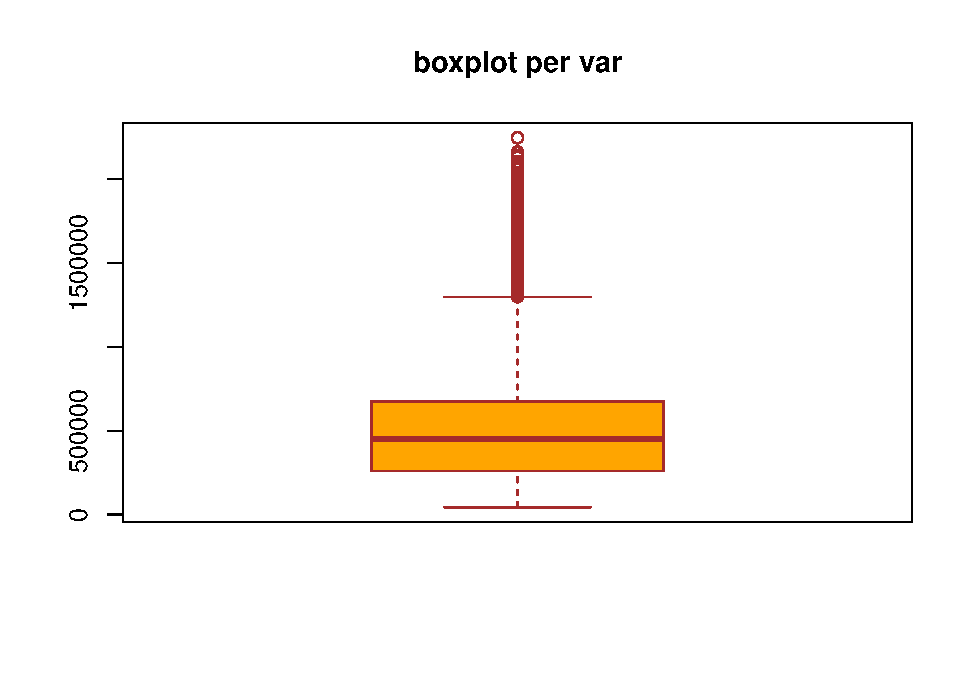
\includegraphics{Presentation_exploratory_analysis_files/figure-latex/unnamed-chunk-4-1.pdf}

\begin{Shaded}
\begin{Highlighting}[]
\CommentTok{#dev.off()}
\end{Highlighting}
\end{Shaded}

\subsubsection{4. Variance and Variance
ratios}\label{variance-and-variance-ratios}

\begin{Shaded}
\begin{Highlighting}[]
\NormalTok{qty <-}\StringTok{ }\KeywordTok{dim}\NormalTok{(data_vars)[}\DecValTok{1}\NormalTok{]}

\CommentTok{# Variance indicators}
\NormalTok{range <-}\StringTok{ }\NormalTok{min_max[}\DecValTok{2}\NormalTok{, ..vars] }\OperatorTok{-}\StringTok{ }\NormalTok{min_max[}\DecValTok{1}\NormalTok{, ..vars]}

\NormalTok{d <-}\StringTok{ }\KeywordTok{as.data.table}\NormalTok{(}\KeywordTok{t}\NormalTok{(}\KeywordTok{apply}\NormalTok{(}\KeywordTok{as.data.table}\NormalTok{(vars), }\DecValTok{1}\NormalTok{, }\ControlFlowTok{function}\NormalTok{(x)\{}\KeywordTok{sum}\NormalTok{(}\KeywordTok{abs}\NormalTok{(data_vars[}\KeywordTok{as.vector}\NormalTok{(}\OperatorTok{!}\KeywordTok{is.na}\NormalTok{(data_vars[, ..x])), ..x] }\OperatorTok{-}\StringTok{ }\KeywordTok{unlist}\NormalTok{(mean_summary[}\DecValTok{1}\NormalTok{,..x]))) }\OperatorTok{/}\StringTok{ }\KeywordTok{sum}\NormalTok{(}\OperatorTok{!}\KeywordTok{is.na}\NormalTok{(data_vars[, ..x]))\})))}
\KeywordTok{colnames}\NormalTok{(d) <-}\StringTok{ }\NormalTok{vars}

\NormalTok{stanDev <-}\StringTok{ }\KeywordTok{as.data.table}\NormalTok{(}\KeywordTok{t}\NormalTok{(}\KeywordTok{apply}\NormalTok{(}\KeywordTok{as.data.table}\NormalTok{(vars), }\DecValTok{1}\NormalTok{, }\ControlFlowTok{function}\NormalTok{(x)\{}\KeywordTok{sd}\NormalTok{(}\KeywordTok{unlist}\NormalTok{(data_vars[}\KeywordTok{as.vector}\NormalTok{(}\OperatorTok{!}\KeywordTok{is.na}\NormalTok{(data_vars[, ..x])), ..x]))\})))}
\KeywordTok{colnames}\NormalTok{(stanDev) <-}\StringTok{ }\NormalTok{vars}


\CommentTok{#Variance ratios (multiplied by 100)}
\NormalTok{Oscillator_ratio <-}\StringTok{ }\NormalTok{(range}\OperatorTok{/}\NormalTok{mean_summary[}\DecValTok{1}\NormalTok{, ..vars]) }\OperatorTok{*}\StringTok{ }\DecValTok{100}
\NormalTok{Linear_variance_ratio <-}\StringTok{ }\NormalTok{(d}\OperatorTok{/}\NormalTok{mean_summary[}\DecValTok{1}\NormalTok{, ..vars]) }\OperatorTok{*}\StringTok{ }\DecValTok{100}
\NormalTok{Variance_ratio <-}\StringTok{ }\NormalTok{(stanDev}\OperatorTok{/}\NormalTok{mean_summary[}\DecValTok{1}\NormalTok{, ..vars]) }\OperatorTok{*}\StringTok{ }\DecValTok{100}

\NormalTok{Overall_Variance_Summary <-}\StringTok{ }\KeywordTok{cbind}\NormalTok{(}\KeywordTok{c}\NormalTok{(}\StringTok{'Range'}\NormalTok{, }\StringTok{'Average Linear_variance'}\NormalTok{, }\StringTok{'Standard Deviation'}\NormalTok{), }\KeywordTok{rbind}\NormalTok{(range, d, stanDev))}
\NormalTok{Overall_Variance_ratios_Summary <-}\StringTok{ }\KeywordTok{cbind}\NormalTok{(}\KeywordTok{c}\NormalTok{(}\StringTok{'Oscillator_ratio'}\NormalTok{, }\StringTok{'Linear_variance_ratio'}\NormalTok{, }\StringTok{'Variance_ratio'}\NormalTok{), }\KeywordTok{rbind}\NormalTok{(Oscillator_ratio, Linear_variance_ratio, Variance_ratio))}

\NormalTok{Overall_Variance_Summary <-}\StringTok{ }\KeywordTok{rbind}\NormalTok{(Overall_Variance_Summary, Overall_Variance_ratios_Summary)}
\KeywordTok{colnames}\NormalTok{(Overall_Variance_Summary)[}\DecValTok{1}\NormalTok{] <-}\StringTok{ 'item'}
\KeywordTok{print}\NormalTok{(Overall_Variance_Summary)}
\end{Highlighting}
\end{Shaded}

\begin{verbatim}
##                       item AMT_INCOME_TOTAL   AMT_CREDIT  AMT_ANNUITY
## 1:                   Range     4.383059e+06 2.200500e+06 178281.00000
## 2: Average Linear_variance     6.746167e+04 2.687951e+05  12152.80068
## 3:      Standard Deviation     1.015226e+05 3.653970e+05  16016.36832
## 4:        Oscillator_ratio     2.456433e+03 4.258424e+02    605.85722
## 5:   Linear_variance_ratio     3.780810e+01 5.201742e+01     41.29920
## 6:          Variance_ratio     5.689714e+01 7.071190e+01     54.42886
##    AMT_GOODS_PRICE REGION_POPULATION_RELATIVE HOUR_APPR_PROCESS_START
## 1:    2.200500e+06                 0.07225500               23.000000
## 2:    2.427241e+05                 0.01073374                2.632769
## 3:    3.367102e+05                 0.01442819                3.278172
## 4:    4.756616e+02               340.41374635              191.549103
## 5:    5.246741e+01                50.56966490               21.926288
## 6:    7.278351e+01                67.97530604               27.301344
\end{verbatim}


\end{document}
